%%%%%%%%%%%%%%%%%%%%%%%%%%%%%%%%%%%%%%%%%%%%%%%%%%%%%%%%%%%%%%%%%%%%
%% I, the copyright holder of this work, release this work into the
%% public domain. This applies worldwide. In some countries this may
%% not be legally possible; if so: I grant anyone the right to use
%% this work for any purpose, without any conditions, unless such
%% conditions are required by law.
%%%%%%%%%%%%%%%%%%%%%%%%%%%%%%%%%%%%%%%%%%%%%%%%%%%%%%%%%%%%%%%%%%%%

\documentclass{beamer}
\usetheme[faculty=phil]{fibeamer}
\usepackage[utf8]{inputenc}
\usepackage[
  main=english, %% By using `czech` or `slovak` as the main locale
                %% instead of `english`, you can typeset the
                %% presentation in either Czech or Slovak,
                %% respectively.
  czech, slovak %% The additional keys allow foreign texts to be
]{babel}        %% typeset as follows:
%%
%%   \begin{otherlanguage}{czech}   ... \end{otherlanguage}
%%   \begin{otherlanguage}{slovak}  ... \end{otherlanguage}
%%
%% These macros specify information about the presentation
\title{Classical Black Holes} %% that will be typeset on the
\subtitle{03. Schwarzschild's Black hole Geometry} %% title page.
\author{Edward Larra\~{n}aga}
%% These additional packages are used within the document:
\usepackage{ragged2e}  % `\justifying` text
\usepackage{booktabs}  % Tables
\usepackage{tabularx}
\usepackage{tikz}      % Diagrams
\usetikzlibrary{calc, shapes, backgrounds}
\usepackage{amsmath, amssymb}
\usepackage{url}       % `\url`s
\usepackage{listings}  % Code listings
\usepackage{siunitx}
\frenchspacing
\begin{document}
  \frame{\maketitle}

  \AtBeginSection[]{% Print an outline at the beginning of sections
    \begin{frame}<beamer>
      \frametitle{Outline for Part \thesection}
      \tableofcontents[currentsection]
    \end{frame}}
    \section{Schwarzschild's Black Hole Geometry}
    
    \subsection{Kruskal Coordinates}
    	\begin{frame}{Schwarzschild's Solution}
    		$$ ds^2 = - \left( 1 - \frac{2M}{r} \right) dt^2 
            + \left( 1 - \frac{2M}{r} \right)^{-1} dr^2 
            + r^2 d\Omega^{2} $$
            \pause
            $$ d\Omega^{2} = d\theta^2 + \sin^2 \theta d\phi^2 $$
            \bigskip
            
            Geometrical units: $ G = c = 1$ 
    	\end{frame}
        
        \begin{frame}{Eddington-Finkelstein Coordinates}
        	$$ (t, r, \theta, \phi) \longrightarrow (v, u, \theta, \phi) $$
            \pause
            $$ v = t + r^* $$
            $$ u = t - r^* $$
            \pause
        	$$ r^{*} = r + 2M \ln\left| \frac{r-2M}{2M}\right| $$
            \pause
            \bigskip
            
            $$ ds^2=-\left(1-\frac{2M}{r}\right)dvdu + r^2 d\Omega^{2} $$
    	\end{frame}
        
        \begin{frame}{Eddington-Finkelstein Coordinates}
            $$ ds^2=-\left(1-\frac{2M}{r}\right)dvdu + r^2 d\Omega^{2} $$
            \pause
            \bigskip
            
			While the original coordinate $r$ takes values in the range $2M < r < \infty$,
the new coordinates $v$ and $u$ take values in the ranges $ -\infty < v < \infty$ and $ -\infty < u < \infty$.
        \end{frame}
        
        \begin{frame}{Eddington-Finkelstein Coordinates}
            $$ ds^2=-\left(1-\frac{2M}{r}\right)dvdu + r^2 d\Omega^{2} $$
            \pause
            \bigskip
            
            $r$ is defined implicitly by the relation
			$$\frac{1}{2}\left(v-u\right)=r^{*}=r+2M\ln\left|\frac{r-2M}{2M}\right|
$$        
        \end{frame}
        
        \begin{frame}{Kruskal Coordinates}
            $$ (v, u, \theta, \phi) \longrightarrow (V, U, \theta, \phi) $$
            \pause
            	\begin{align*}
					V & =  e^{\frac{v}{4M}}\\
					U & =  -e^{-\frac{u}{4M}}
				\end{align*}
            \pause
            \bigskip
            
            $$ ds^2 = -\frac{32M^3}{r} e^{-\frac{r}{2M}} dVdU + r^2 d\Omega^{2} $$
        \end{frame}
        
    	\begin{frame}{Kruskal Coordinates}
            $$ ds^2 = -\frac{32M^3}{r} e^{-\frac{r}{2M}} dVdU + r^2 d\Omega^{2} $$
            \pause
            
            $r$ is defined by the relation

			$$ UV =  -\left[\frac{r-2M}{2M}\right] e^{\frac{r}{2M}} $$
        \end{frame}
        
	\subsection{Kruskal Diagram}
        \begin{frame}{Kruskal Diagram}
            $$ UV =  -\left[\frac{r-2M}{2M}\right] e^{\frac{r}{2M}} $$
            \pause
            \begin{itemize}
            \item $r=2M$ is represented by the set $\left\{ U=0\right\} \cup\left\{V=0\right\} $
            \pause
            \item The exterior region $r>2M$ is represented by the new coordinates in the range $U<0$ and $V>0$
            \pause
            \item However, the metric tensor is regular at $r=2M$ and therefore we can analytically extend the coordinates to include the regions with $U>0$ and $V<0$.
            \end{itemize}
      	\end{frame}
        
        \begin{frame}{Kruskal Diagram}
        	\begin{center}
				\begin{figure}
				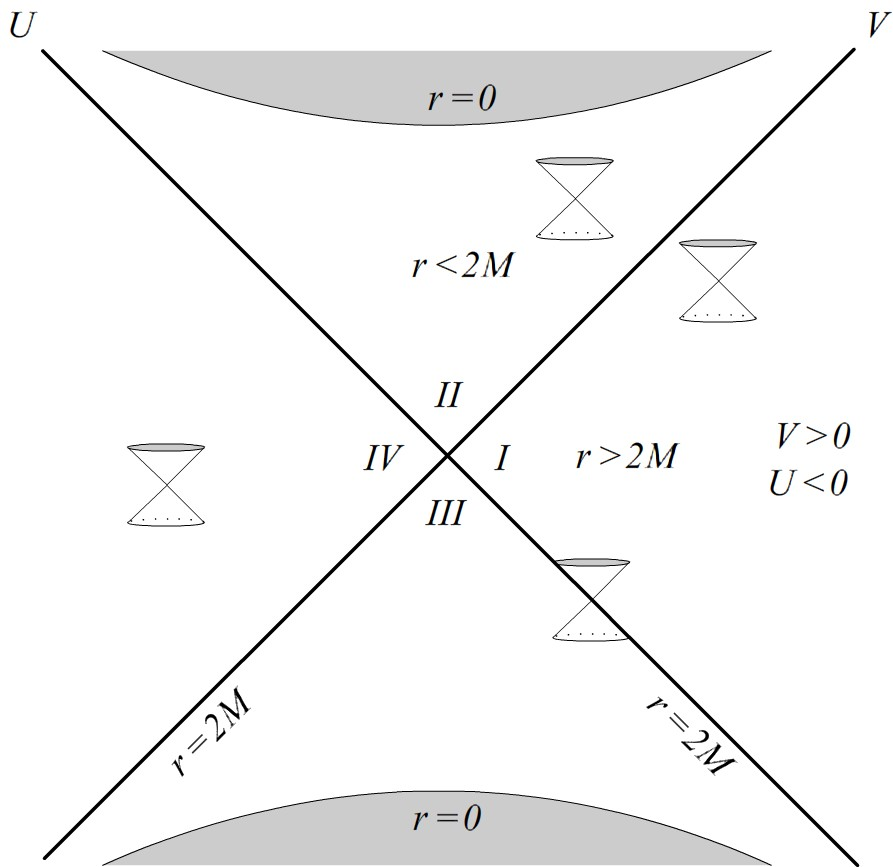
\includegraphics[scale=0.75] {fig4.jpg}
				\end{figure}
			\end{center}	
        \end{frame}
        
        \begin{frame}{Kruskal Hypersurfaces}
			$$ UV =  -\left[\frac{r-2M}{2M}\right] e^{\frac{r}{2M}} $$
            \pause
            \bigskip
            
            $r = \textrm{constant}$ gives the hypersurfaces
            $$ UV = \textrm{constant} $$
            \pause
            \centering {(Hyperbolae)}
        \end{frame}
        
        \begin{frame}{Kruskal Hipersurfaces}
			$$ \frac{V}{U}=e^{-\frac{t}{2M}} $$
            \pause
            \bigskip
            
            $t = \textrm{constant}$ gives the hypersurfaces
            $$ \frac{V}{U} = \textrm{constant} $$
            \pause
            \centering {(Straight Lines)}
        \end{frame}
        
        \begin{frame}{Kruskal Diagram}
        	\begin{center}
				\begin{figure}
				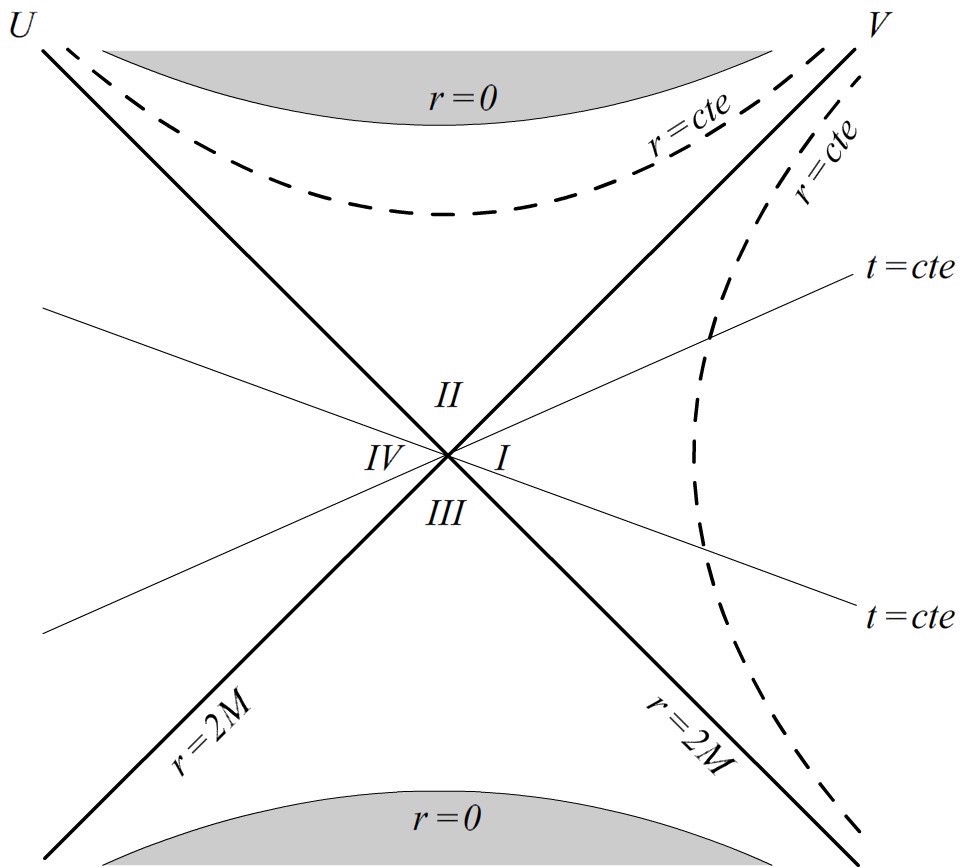
\includegraphics[scale=0.24] {fig5.jpg}
				\end{figure}
			\end{center}	
        \end{frame}
        
        \begin{frame}{Kruskal Hipersurfaces}
			
            Isometry of Kruskal Manifold:
            $$\left(U,V\right)\longrightarrow\left(-U,-V\right)$$
            
			i.e. region IV is indeed the time inverse of region I
            \pause
            \bigskip
            
            This isometry has the \emph{fixed point}  $\left\{ U=0\right\} \cup\left\{V=0\right\} $ or equivalently $r=2M$
        \end{frame}
        
        \begin{frame}{Kruskal Diagram}
        	\begin{center}
				\begin{figure}
				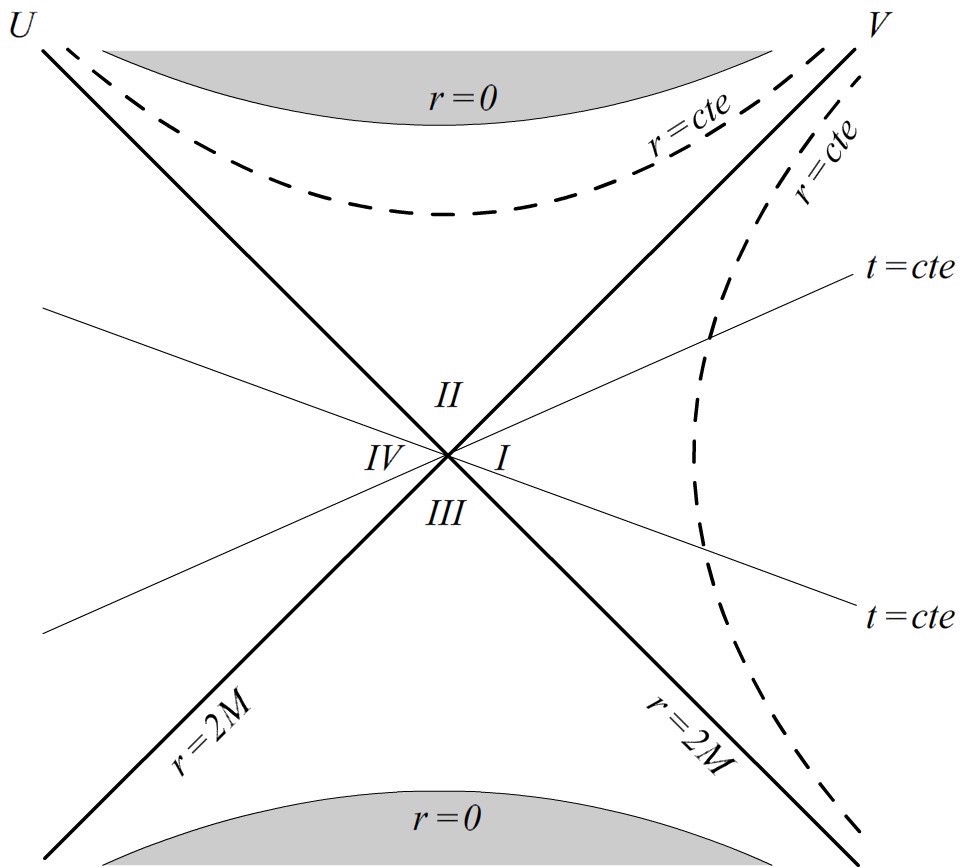
\includegraphics[scale=0.24] {fig5.jpg}
				\end{figure}
			\end{center}	
        \end{frame}
    
        \begin{frame}{Timelike Killing Vector Field}
			\begin{itemize}
			\item Schwarzschild's Coordinates:\\
            	$\xi = \frac{\partial}{\partial t}$\\
            	\pause
                Corresponds to the invariance under $t\longrightarrow t + k$
                \pause
            \bigskip
            
            \item Kruskal Coordinates: \\
            $ V \longrightarrow  V e^{\frac{k}{4M}} $ \\
			$ U \longrightarrow  U e^{-\frac{k}{4M}}$
			\end{itemize}
        \end{frame}
        
 	\subsection{Timelike Killing Vector Field}       
        \begin{frame}{Timelike Killing Vector Field}
			\begin{itemize}
			\item Kruskal Coordinates: \\
            Infinitesimal version of the transformation is\\
            $ \delta U  \longrightarrow  -\frac{k}{4M}U$\\
			$ \delta V  \longrightarrow  \frac{k}{4M}V$
            \pause
            \bigskip
            
            $\xi = \frac{1}{4M} \left[ V \frac{\partial}{\partial V} - U \frac{\partial}{\partial U} \right]$
			\end{itemize}
        \end{frame}
        
        \begin{frame}{Timelike Killing Vector Field}
            $$\xi = \frac{1}{4M} \left[ V \frac{\partial}{\partial V} - U \frac{\partial}{\partial U} \right]$$
            \bigskip
            
            $$\xi^{2} = - \left( 1 - \frac{2M}{r} \right)$$

			\begin{itemize}
			\item $\xi$ is timelike in regions I and IV
        	\pause 
        	\item $\xi$ is spacelike in regions II and III
        	\pause 
        	\item $\xi$ is a null vector at the surface $r=2M$
			\end{itemize} 
		\end{frame}
        
        \begin{frame}{Kruskal Diagram}
        	\begin{center}
				\begin{figure}
				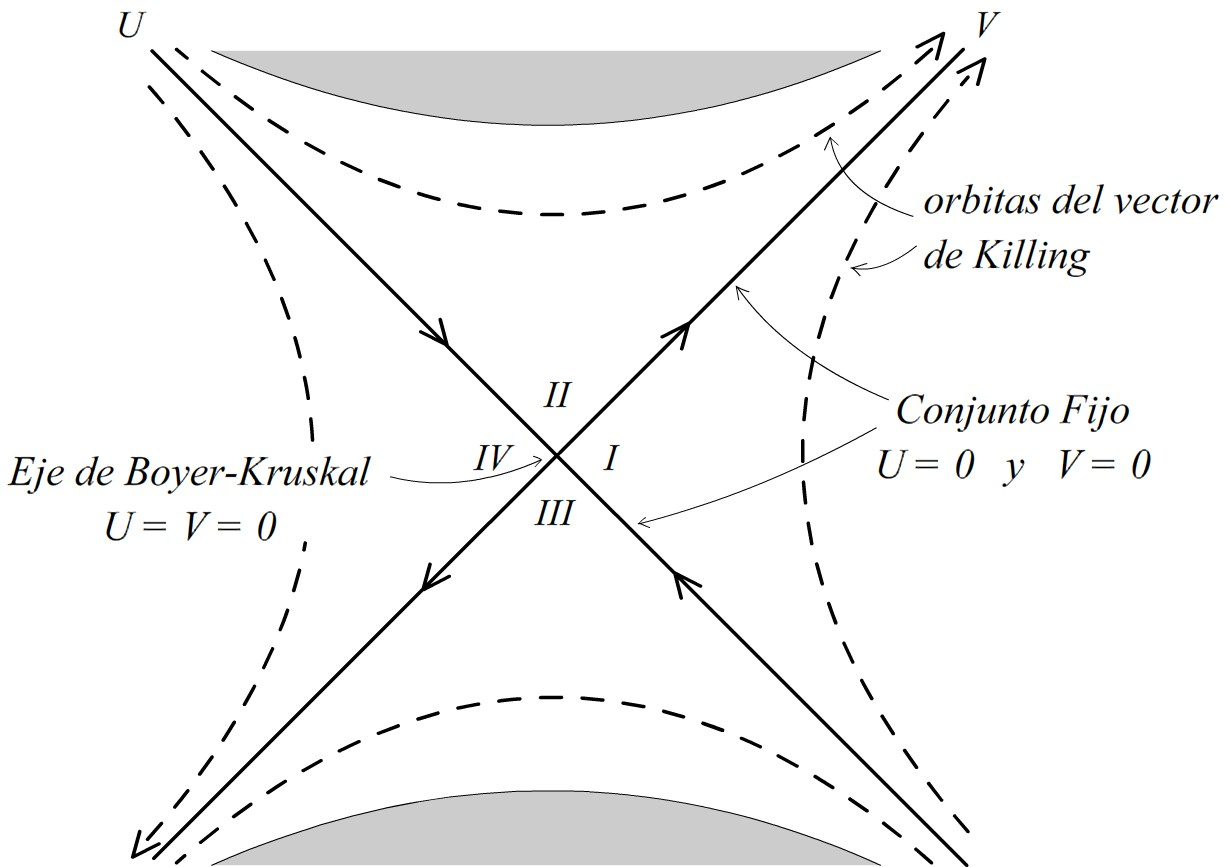
\includegraphics[scale=0.75] {fig7.jpg}
				\end{figure}
			\end{center}	
        \end{frame}
        
        \begin{frame}{Back to Timelike and Spacelike Coordinates}
            $$ (V, U, \theta, \phi) \longrightarrow (T, X, \theta, \phi) $$
            \pause
            	\begin{align*}
					T & = \frac{1}{2}\left(V-U\right)\\
					X & = \frac{1}{2}\left(V+U\right),
				\end{align*}
            \pause
            \bigskip
            
            $$ ds^2 = \frac{32M^{3}}{r}e^{-\frac{r}{2M}}\left[ -dT^2 + dX^2 \right] + r^2 d\Omega^{2} $$
        \end{frame}
        
        \begin{frame}{Kruskal Diagram}
        	\begin{center}
				\begin{figure}
				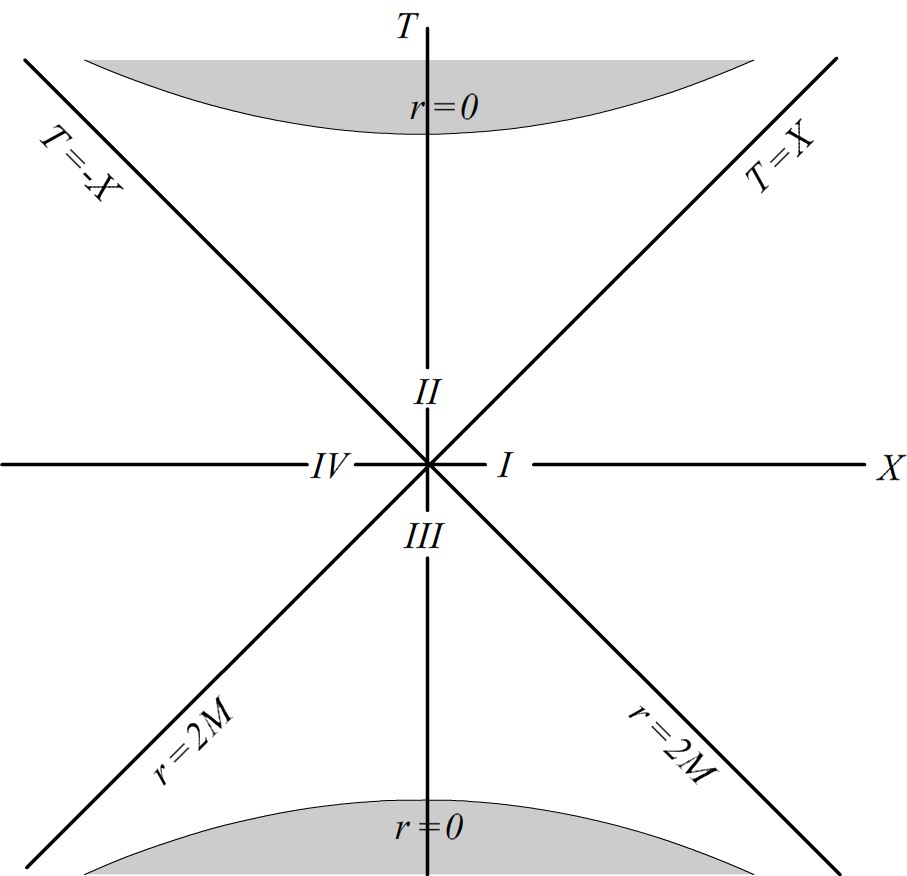
\includegraphics[scale=0.75] {fig6.jpg}
				\end{figure}
			\end{center}	
        \end{frame}
        
        \begin{frame}{Dynamical Behavior of the Manifold}
        	\begin{center}
				\begin{figure}
				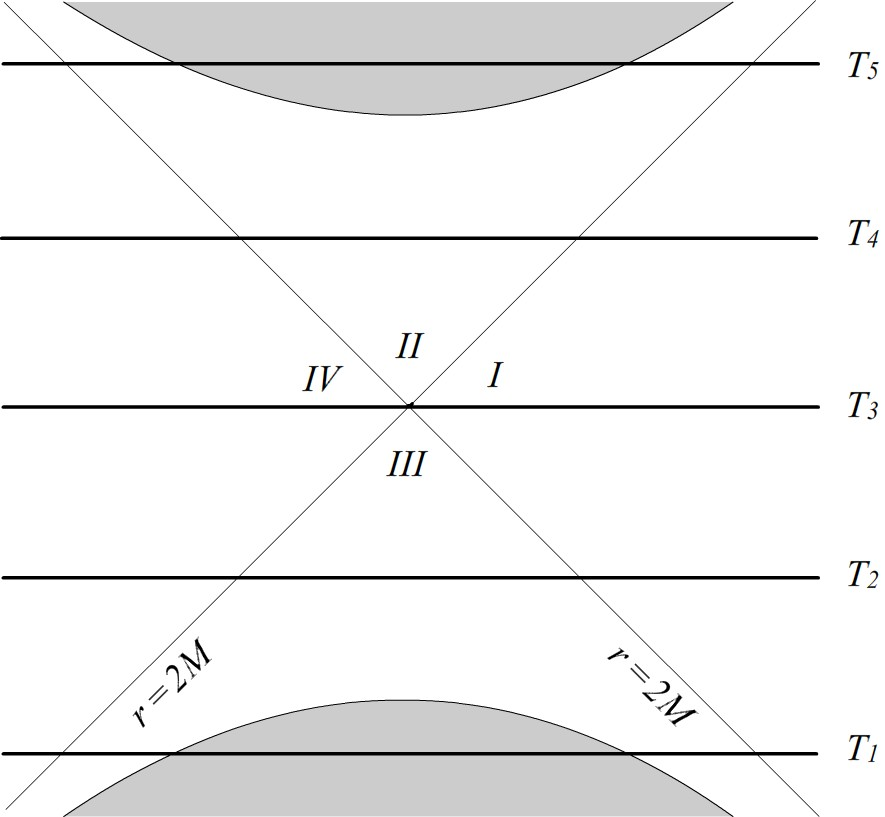
\includegraphics[scale=0.75] {fig9.jpg}
				\end{figure}
			\end{center}	
        \end{frame}
        
        \begin{frame}{Dynamical Behavior of the Manifold}
        	\begin{center}
				\begin{figure}
				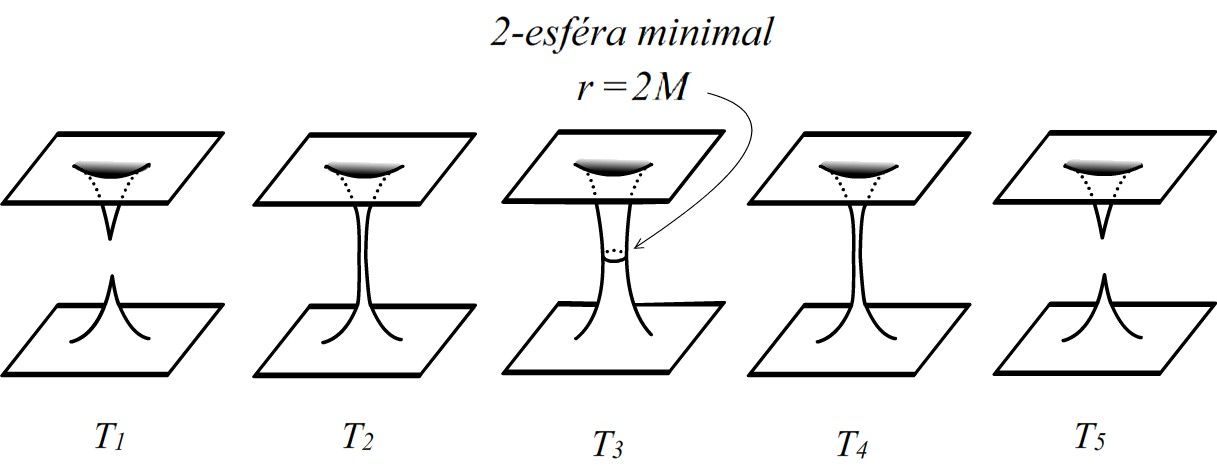
\includegraphics[scale=0.75] {fig10.jpg}
				\end{figure}
			\end{center}	
        \end{frame}
      
	\subsection{Isotropic Coordinates}
    	\begin{frame}{Isotropic Coordinates}
    		$$ (t, r, \theta, \phi) \longrightarrow (t, \rho, \theta, \phi) $$
            such that the line element becomes conformally flat in its spatial part:
            \pause
        	$$ ds^2=-\left( 1 - \frac{2M}{r} \right) dt^2 + 	
            \omega^2\left( \rho \right) \left[ d\rho^{2} + \rho^{2} d\Omega^{2} \right] $$
    	\end{frame}
        
        \begin{frame}{Isotropic Coordinates}
        	$$ ds^2=-\left( 1 - \frac{2M}{r} \right) dt^2 + 	
            \omega^2\left( \rho \right) \left[ d\rho^{2} + \rho^{2} 
            d\Omega^{2} \right] $$
            This requires that
            \pause
            $$\omega^2\left(\rho\right)\rho^2 = r^2$$
            \pause
            $$ \frac{dr^2}{\left( 1 - \frac{2M}{r} \right)} = \omega^2 d\rho^2 $$

            \bigskip
            
            $$\Longrightarrow r = \left( 1 + \frac{M}{2\rho} \right)^2 \rho$$
    	\end{frame}
        
        \begin{frame}{Isotropic Coordinates}
        	$$ ds^2 = -\frac{\left(1-\frac{M}{2\rho} \right)^2}{\left(1+\frac{M}
            {2\rho}\right)^2}dt^2 + \left(1+\frac{M}{2\rho}\right)^4 
            \left[d\rho^2 + \rho^2 d\Omega^2 \right]$$
    	\end{frame}
        
        \begin{frame}{Isotropic Coordinates}
        	$$ r = \left( 1 + \frac{M}{2\rho} \right)^2 \rho $$
            \pause
            Isometry
			$$ \rho \longrightarrow \frac{M^{2}}{4\rho} $$
            \pause
            \bigskip
            
            Fixed point at $\rho=\frac{M}{2}$ corresponding to the 2-sphere of radius $r=2M$
    	\end{frame}
        
        \begin{frame}{Isotropic Coordinates Isometry}
        	\begin{center}
				\begin{figure}
				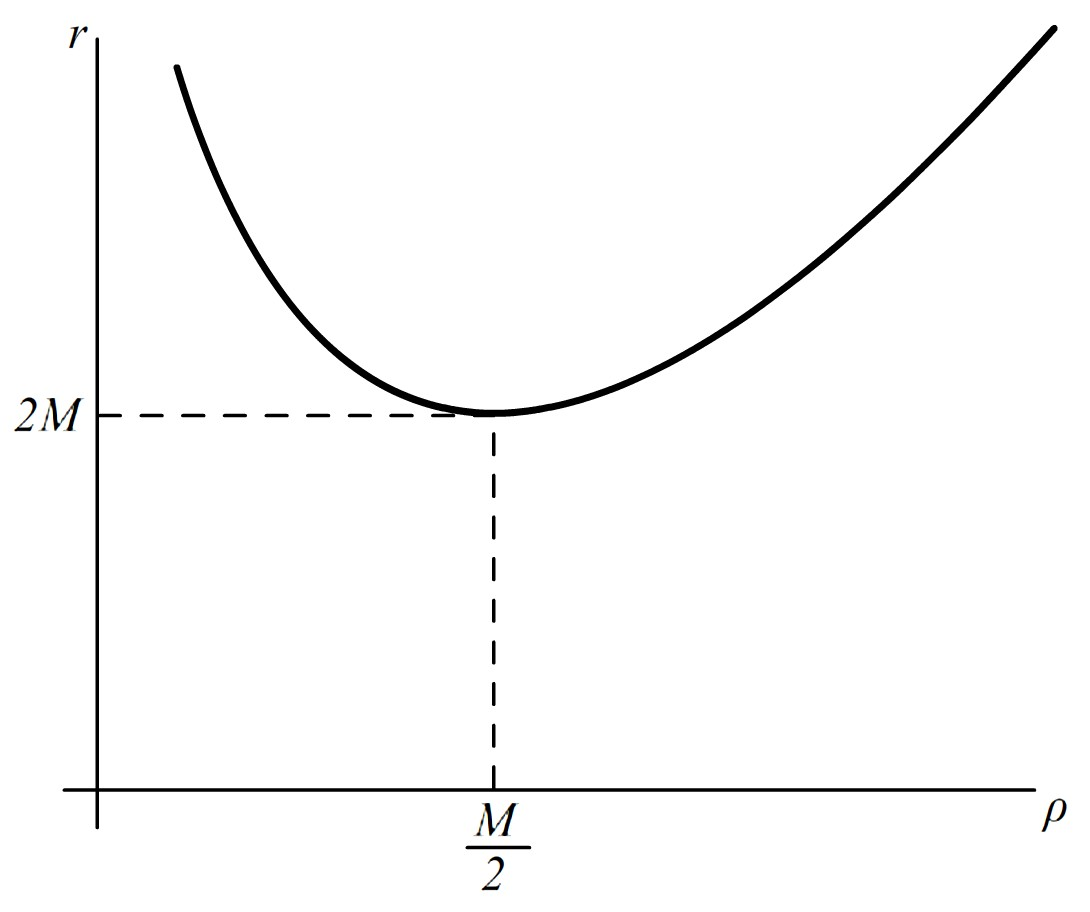
\includegraphics[scale=0.75] {fig8.jpg}
				\end{figure}
			\end{center}	
        \end{frame}
        
        \begin{frame}{Isotropic Coordinates Isometry}
        	\begin{center}
				\begin{figure}
				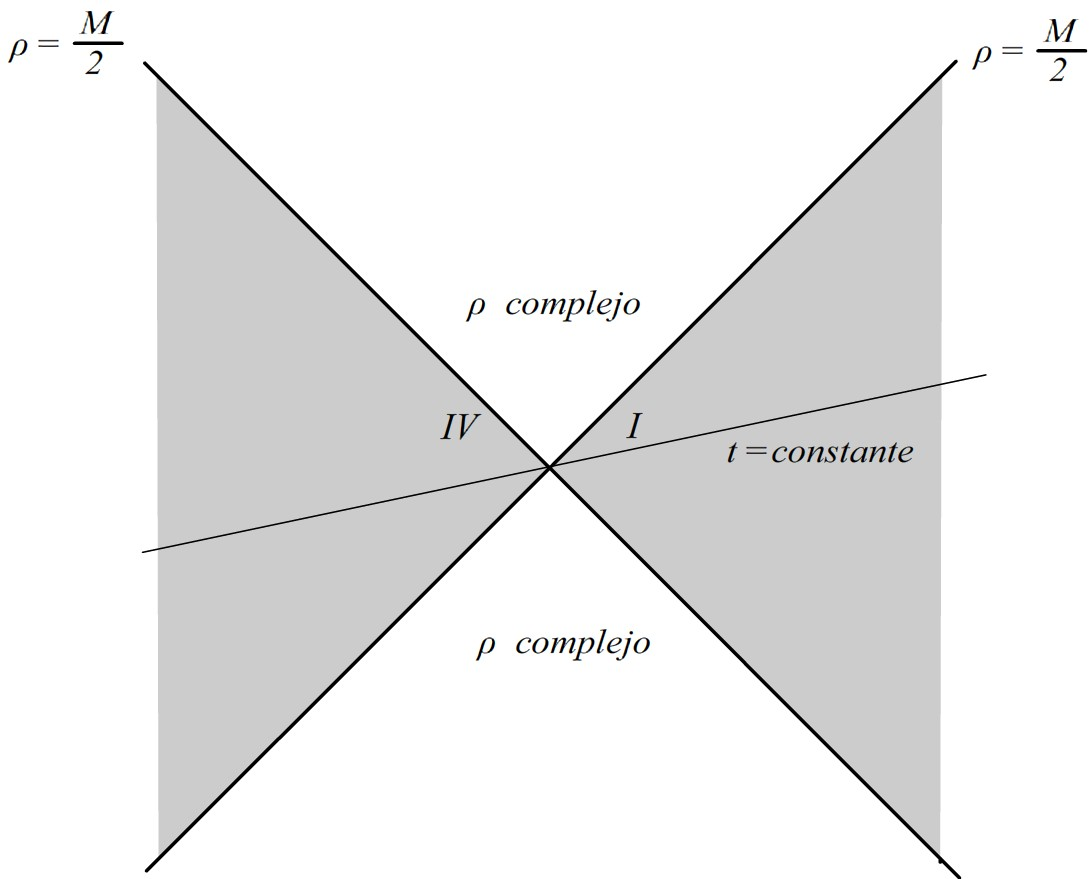
\includegraphics[scale=0.75] {fig8a.jpg}
				\end{figure}
			\end{center}	
        \end{frame}
        
        \begin{frame}{Cartesian Coordinates}
        	$$ ds^2 = -\frac{\left(1-\frac{M}{2\rho}\right)^2}
            {\left(1+\frac{M}{2\rho}\right)^{2}} dt^2 + \left(1+\frac{M}{2\rho}\right)^4 
            \left[dx^2 + dy^2 + dz^2\right]$$
            
            $$r = \sqrt{x^{2}+y^{2}+z^{2}} = \rho\left(1+\frac{M}{2\rho}\right)^2$$
    	\end{frame}
        
        \begin{frame}{Killing Vectors in Cartesian Coordinates}
        	\pause
        	\begin{align*}
				\xi &= \frac{\partial}{\partial t}\\
				\zeta_1 &= x\frac{\partial}{\partial y}-y\frac{\partial}{\partial x}\\
				\zeta_2 &= y\frac{\partial}{\partial z}-z\frac{\partial}{\partial y}\\
				\zeta_3 &= z\frac{\partial}{\partial x}-x\frac{\partial}{\partial z}
			\end{align*}
       	\end{frame}


  	\subsection{Carter-Penrose Diagrams}
    
    	\begin{frame}
        	\Large
			{Carter-Penrose Diagrams}
		\end{frame}
        
  		\begin{frame}{Compactification}
  			$$ ds^2\longrightarrow d\tilde{s}^2 = \omega^2 \left( x^\mu \right) ds^2$$
            \pause
            \bigskip
            
            \centering
            {$\omega \longrightarrow 0$ when $x^i\longrightarrow\infty$}
  		\end{frame}
        
    	\begin{frame}{Minkowski's Spacetime}
			$$ ds^2 = -dt^2 + dr^2+r^2 d\Omega^2 $$
			\pause
			Range of $t$ and $r$ 
				$$ -\infty <   t  <\infty$$
             	$$0\leq r <\infty$$
    	\end{frame}
        
    	\begin{frame}{Minkowski's Spacetime in Null Coordinates}
    		Null coordinates:
			\begin{align*}
				v &=  t+r\\
				u &=  t-r
			\end{align*}
			\pause
			$$ ds^2= - dvdu + \frac{ \left( u-v \right)^2}{4} d\Omega^2 $$
            \pause
			Ranges of $v$ and $u$
            	$$ -\infty <  v < \infty$$
                $$ -\infty <  u < \infty$$
    	\end{frame}
        
        \begin{frame}{Minkowski's Spacetime in Null Coordinates}
			$$ ds^2= - dvdu + \frac{ \left( u-v \right)^2}{4} d\Omega^2 $$
			Ranges of $v$ and $u$
            	$$ -\infty <  v < \infty$$
                $$ -\infty <  u < \infty$$
            \pause
			Extra Condition: 
            $$r=\frac{1}{2}\left(v-u\right)\geq0 \Rightarrow u\leq v $$.
    	\end{frame}
        
        \begin{frame}{Compactification of Minkowski's Spacetime}
			$$ ds^2= - dvdu + \frac{ \left( u-v \right)^2}{4} d\Omega^2 $$
            \pause
            \begin{align*}
				v &=  \tan V\\
				u &=  \tan U
			\end{align*}
    	\end{frame}
        
        \begin{frame}{Compactification of Minkowski's Spacetime}
        	\begin{center}
				\begin{figure}
				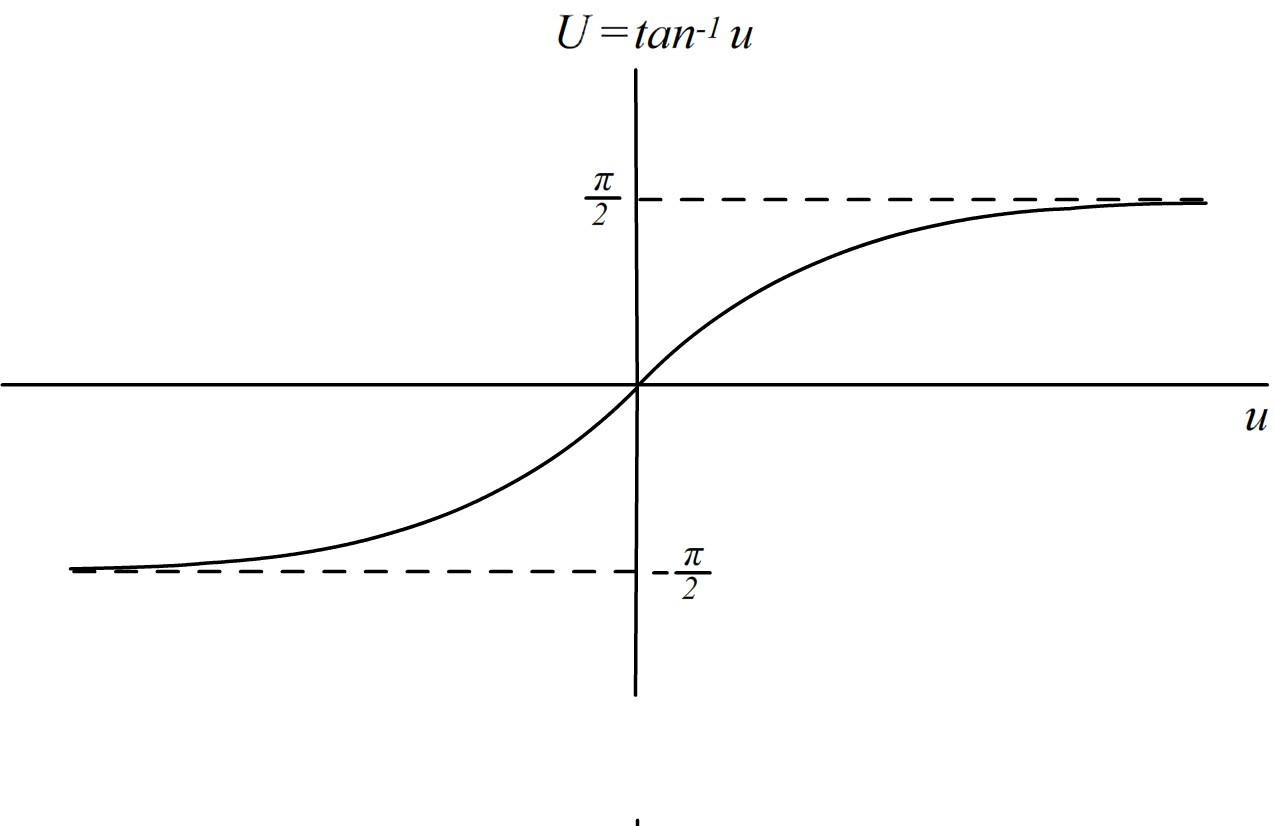
\includegraphics[scale=0.75] {fig12.jpg}
				\end{figure}
			\end{center}	
        \end{frame}
        
    	\begin{frame}{Compactification of Minkowski's Spacetime}
			$$ ds^2= - dvdu + \frac{ \left( u-v \right)^2}{4} d\Omega^2 $$
            \begin{align*}
				v &=  \tan V\\
				u &=  \tan U
			\end{align*}
            \pause
            $$ds^2 = \frac{1}{\left(2\cos V\cos U\right)^{2}} \left[ -4dVdU + \sin^2 \left( V - U \right) d\Omega^2 \right]$$
    	\end{frame}
        
        \begin{frame}{Compactification of Minkowski's Spacetime}
            $$ds^2 = \frac{1}{\left(2\cos V\cos U\right)^{2}} \left[ -4dVdU + \sin^2 \left( V - U \right) d\Omega^2 \right]$$
            \pause
            $$-\frac{\pi}{2}<  V  <\frac{\pi}{2}$$
            $$-\frac{\pi}{2}<  U  <\frac{\pi}{2}$$
            \pause
            \bigskip
            
            \centering
            {Together with the condition $U\leq V$}
    	\end{frame}
        
        \begin{frame}{Compactification of Minkowski's Spacetime}
            $$ds^2 = \frac{1}{\left(2\cos V\cos U\right)^{2}} \left[ -4dVdU + \sin^2 \left( V - U \right) d\Omega^2 \right]$$
            \pause
            $$\omega = 2\cos V\cos U$$
            \pause
            It satisfies $\omega\longrightarrow0$ when $\left| V \right| \longrightarrow \frac{\pi}{2}$ or when $\left|U\right|\longrightarrow\frac{\pi}{2}$\\
			\pause
			$$ d\tilde{s}^2 = \omega^2 ds^2 = -4dVdU + \sin^2 \left( V - U\right) d\Omega^2 $$
    	\end{frame}
        
        \begin{frame}{Compactification of Minkowski's Spacetime}
			$$ d\tilde{s}^2 = \omega^2 ds^2 = -4dVdU + \sin^2 \left( V - U\right) d\Omega^2 $$
            \pause
            \begin{align*}
				\eta &= V+U\\
				\chi &= V-U
			\end{align*}
            \pause
            $$ d\tilde{s}^2 = -d\eta^2 + d\chi^2 + \sin^2 \chi d\Omega^2 $$
    	\end{frame}
       	
        \begin{frame}{Compactification of Minkowski's Spacetime}
            $$ d\tilde{s}^2 = -d\eta^2 + d\chi^2 + \sin^2 \chi d\Omega^2 $$
            \pause
            $$-\pi<  \eta  <\pi$$
			$$0\leq  \chi  <\pi$$
    	\end{frame}

		\begin{frame}
        	\tiny{
        	\begin{table}[h]
			\begin{centering}
			\begin{tabular}{|c|c|c|c|c|}
			\hline 
			infinite & $\left(t,r\right)$ & $\left(v,u\right)$ & $\left(V,U\right)$ & 							$\left(\eta,\chi\right)$\tabularnewline
			\hline 
			\hline 
			$i_{0}$ : spatial & $\begin{cases}
			t & \mbox{finite}\\
			r & \rightarrow+\infty
			\end{cases}$ & $\begin{cases}
			v & \rightarrow+\infty\\
			u & \rightarrow-\infty
            \end{cases}$ & $\begin{cases}
            V & =\frac{\pi}{2}\\
            U & =-\frac{\pi}{2}
            \end{cases}$ & $\begin{cases}
            \eta & =0\\
            \chi & =\pi
            \end{cases}$\tabularnewline
            \hline 
            $i_{+}$ : temporal future & $\begin{cases}
            t & \rightarrow\infty\\
            r & \mbox{finite}
            \end{cases}$ & $\begin{cases}
            v & \rightarrow+\infty\\
            u & \rightarrow+\infty
            \end{cases}$ & $\begin{cases}
            V & =\frac{\pi}{2}\\
            U & =\frac{\pi}{2}
            \end{cases}$ & $\begin{cases}
            \eta & =\pi\\
            \chi & =0
            \end{cases}$\tabularnewline
            \hline 
            $i_{-}$ : temporal past & $\begin{cases}
            t & \rightarrow-\infty\\
            r & \mbox{finite}
            \end{cases}$ & $\begin{cases}
            v & \rightarrow-\infty\\
            u & \rightarrow-\infty
            \end{cases}$ & $\begin{cases}
            V & =-\frac{\pi}{2}\\
            U & =-\frac{\pi}{2}
            \end{cases}$ & $\begin{cases}
            \eta & =-\pi\\
            \chi & =0
            \end{cases}$\tabularnewline
            \hline 
            $\mathcal{I}_{+}$ : null future & $\left\{ \begin{array}{c}
            t\rightarrow+\infty\\
            r\rightarrow+\infty\\
            t-r\mbox{ finite}
            \end{array}\right.$ & $\begin{cases}
            v & \rightarrow+\infty\\
            u & \mbox{finite}
            \end{cases}$ & $\left\{ \begin{array}{c}
            V=\frac{\pi}{2}\\
            -\frac{\pi}{2}<U<\frac{\pi}{2}
            \end{array}\right.$ & $\left\{ \begin{array}{c}
            \eta=\pi-\chi\\
            0<\chi<\pi
            \end{array}\right.$\tabularnewline
            \hline 
            $\mathcal{I}_{-}$ : null past & $\left\{ \begin{array}{c}
            t\rightarrow-\infty\\
            r\rightarrow+\infty\\
            t+r\mbox{ finite}
            \end{array}\right.$ & $\begin{cases}
            v & \mbox{finite}\\
            u & \rightarrow-\infty
            \end{cases}$ & $\left\{ \begin{array}{c}
            -\frac{\pi}{2}<V<\frac{\pi}{2}\\
            U=-\frac{\pi}{2}
            \end{array}\right.$ & $\left\{ \begin{array}{c}
            \eta=-\pi+\chi\\
            0<\chi<\pi
            \end{array}\right.$\tabularnewline
            \hline 
			\end{tabular}
			\par\end{centering}
			\end{table}}
        \end{frame}
        
        \begin{frame}{Carter-Penrose Diagram for Minkowski's spacetime}
        	\begin{center}
				\begin{figure}
				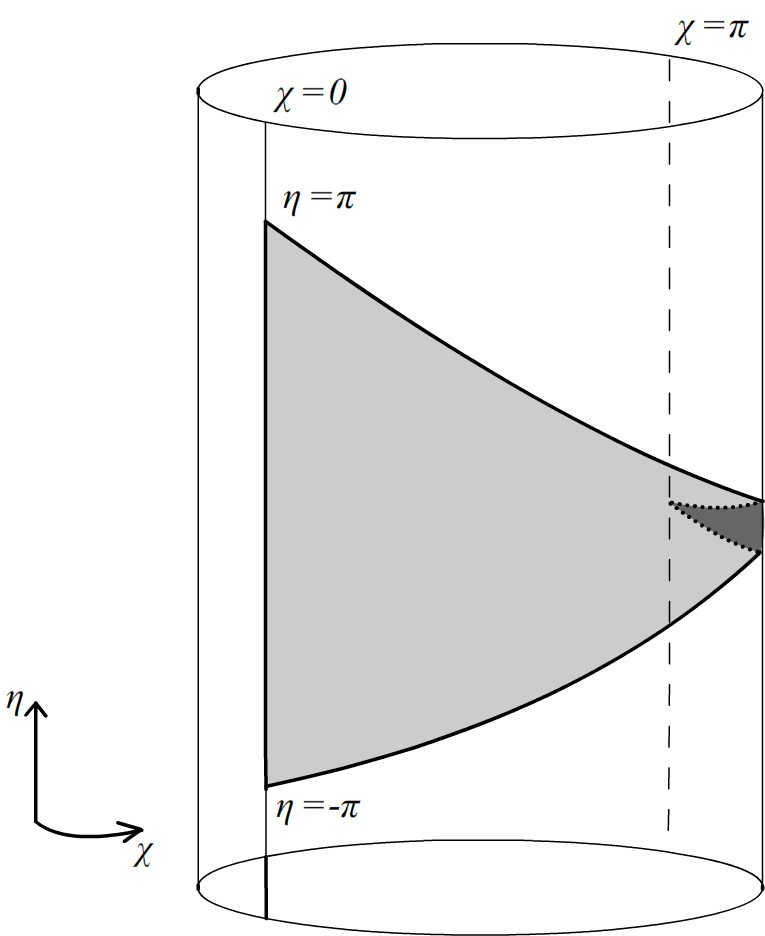
\includegraphics[scale=0.75] {fig13.jpg}
				\end{figure}
			\end{center}	
        \end{frame}
        
        \begin{frame}{Carter-Penrose Diagram for Minkowski's spacetime}
        	\begin{center}
				\begin{figure}
				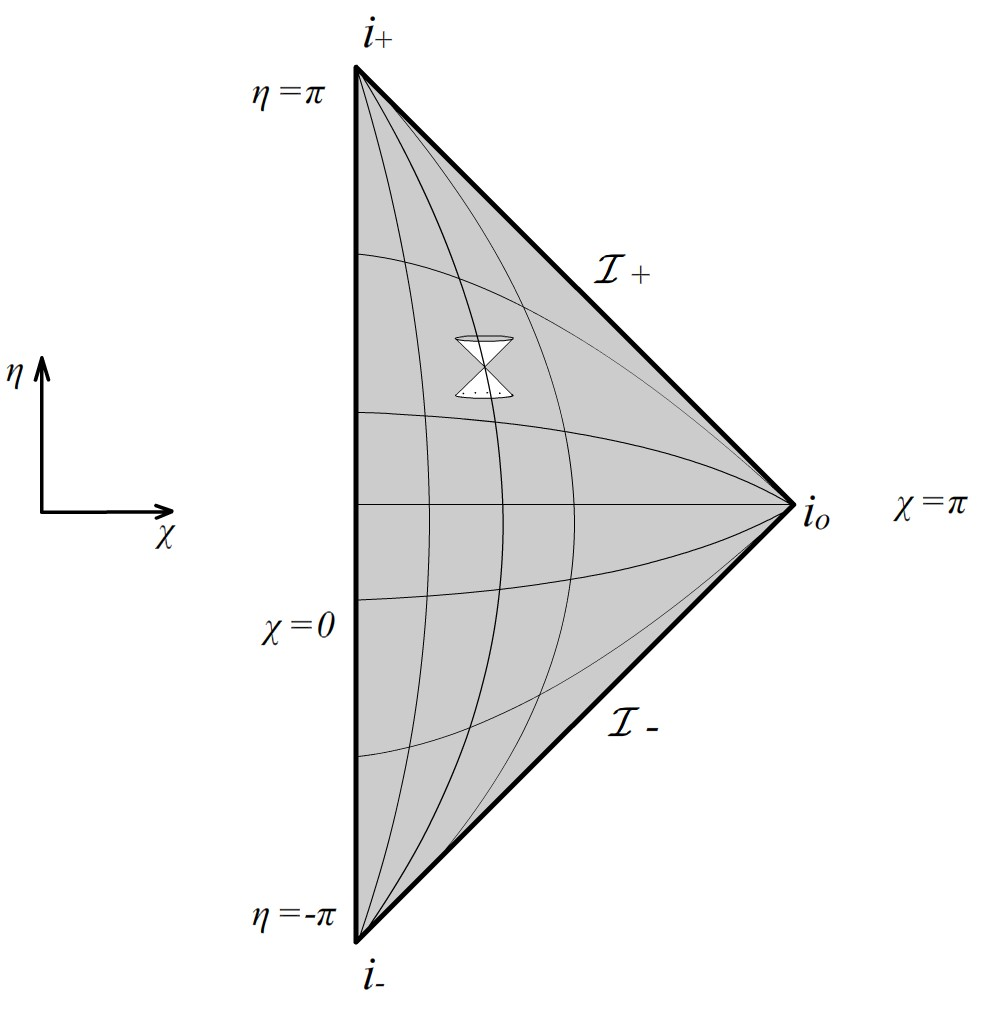
\includegraphics[scale=0.75] {fig15.jpg}
				\end{figure}
			\end{center}	
        \end{frame}
		
        \begin{frame}{Kruskal Spacetime}
        	$$ ds^2 = -\left( 1 - \frac{2M}{r} \right) dvdu + r^2 d\Omega^2 $$
			\pause
			$$ -\infty<  v  <\infty $$
			$$ -\infty<  u  <\infty $$
        \end{frame}
        
        \begin{frame}{Compactification of Kruskal Spacetime}
        	$$ ds^2 = -\left( 1 - \frac{2M}{r} \right) dvdu + r^2 d\Omega^2 $$
			\pause
			$$ v  =  \tan V $$
			$$ u  =  \tan U $$
            \pause
            $$ ds^2 = \frac{1}{\left(2\cos V\cos U\right)^2}\left[-4\left(1-\frac{2M}{r}\right)dVdU + 4r^2 \cos^2 V\cos^2U d\Omega^2 \right]$$
        \end{frame}
        
        \begin{frame}{Compactification of Kruskal Spacetime}
        	$$ ds^2 = \frac{1}{\left(2\cos V\cos U\right)^2}\left[-4\left(1-\frac{2M}{r}\right)dVdU + 4r^2 \cos^2 V\cos^2U d\Omega^2 \right]$$
			\pause
			$$ -\frac{\pi}{2}<  V  <\frac{\pi}{2}$$
			$$ -\frac{\pi}{2}<  U  <\frac{\pi}{2}$$
        \end{frame}
        
        \begin{frame}{Compactification of Kruskal Spacetime}
        	$$ ds^2 = \frac{1}{\left(2\cos V\cos U\right)^2}\left[-4\left(1-\frac{2M}{r}\right)dVdU 
            + 4r^2 \cos^2 V\cos^2U d\Omega^2 \right]$$
			\pause
			$$ r^{*} = \frac{1}{2} \left( v - u \right) = 
            \frac{ \sin\left(V-U\right) }{2\cos V\cos U}$$
            \pause
            \bigskip
            
            \small{
            $$ds^{2}=\frac{1}{\left(2\cos V\cos U\right)^{2}}
            \left[-4\left(1-\frac{2M}{r}\right)dVdU
            +\left(\frac{r}{r^{*}}\right)^{2}\sin^{2}\left(V-U\right)d\Omega^{2}\right]$$}
        \end{frame}
        
        \begin{frame}{Compactification of Kruskal Spacetime}
        	\small{
            $$ds^{2}=\frac{1}{\left(2\cos V\cos U\right)^{2}}\left[-4\left(1-\frac{2M}{r}\right)dVdU+\left(\frac{r}{r^{*}}\right)^{2}\sin^{2}\left(V-U\right)d\Omega^{2}\right]$$}
            \pause
            $$\omega=2\cos V\cos U$$
            \pause
            $$d\tilde{s}^{2}=\omega^{2}ds^{2}=-4\left(1-\frac{2M}{r}\right)dVdU+\left(\frac{r}{r^{*}}\right)^{2}\sin^{2}\left(V-U\right)d\Omega^{2}$$
        \end{frame}
        
        \begin{frame}{Compactification of Kruskal Spacetime}
        	$$d\tilde{s}^{2}=-4\left(1-\frac{2M}{r}\right)dVdU+\left(\frac{r}{r^{*}}\right)^{2}\sin^{2}\left(V-U\right)d\Omega^{2}$$
        \end{frame}
        
        \begin{frame}{Carter-Penrose Diagram for Kruskal Spacetime}
        	\begin{center}
				\begin{figure}
				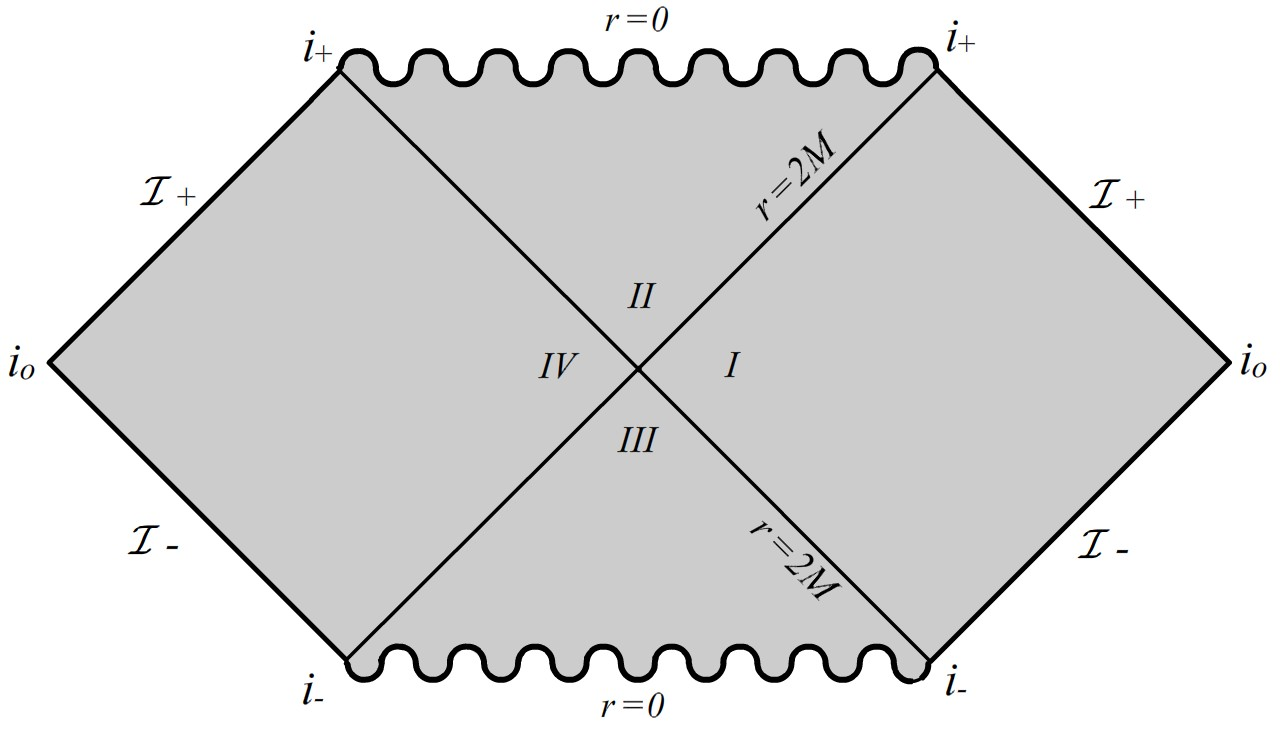
\includegraphics[scale=0.75] {fig17.jpg}
				\end{figure}
			\end{center}	
        \end{frame}


	\section{Hypersurfaces}    
  	\begin{darkframes}
        
        \begin{frame}{Hypersurfaces}
        	\begin{itemize}
            \item $\Sigma$: 3-dimensional submanifold that can be timelike, null or spacelike
            \pause
            \item $\Phi\left(x\right)$ is a smooth function of the coordinates $x^{\mu}$
            \pause
            \item $\Phi\left(x\right)=\textrm{constant}$ defines a family of hypersurfaces 
            \pause
            \item $\partial_{\mu}\Phi$ is normal to the hypersurfaces
        	\end{itemize}
            
        \end{frame}
        
        \begin{frame}{Normal Vector to a Hypersurface}
        	\begin{equation*}
            	\mathbf{n} =	N\left(\partial_{\mu}\Phi\right)\partial^{\mu}	=	
                Ng^{\mu\nu}\partial_{\mu}\Phi\partial_{\nu},\label{eq:vectorNormal}
			\end{equation*}\\
            \pause
 			$N=N\left(x^{\mu}\right)$ is an arbitrary ''normalization'' function.
            \pause
			\begin{equation*}
				n^{2}=n^{\mu}n_{\mu} = \left\{ \begin{array}{c}
				1\\
				-1\\
				0
				\end{array}\right.\begin{array}{c}
				\mbox{if }\Sigma\mbox{ is timelike}\\
				\mbox{if }\Sigma\mbox{ is spacelike}\\
				\mbox{if }\Sigma\mbox{ is null.}
				\end{array}
			\end{equation*}
        \end{frame}
        
    	\begin{frame}{Tangent Vector to a hypersurface}
        	The vector $ t^{\mu} $ is called a \textit{Tangent Vector} to the hypersurface if
    		$$ t^{\mu}n_{\mu}=0 $$
    	\end{frame}
	
    \subsection{Null Hypersurfaces}
    	\begin{frame}{Null Hypersurfaces}
    		\begin{itemize}
    		\item A hypersurface $\mathcal{N}$ is called \emph{null hypersurface} if its normal vector satisfies
			$$ n^{2}=n_{\mu}n^{\mu}=0$$
            \pause
            \item Since the normal vector is orthogonal to itself, $\mathbf{n}$ is also a tangent vector. 
			\pause
            \item $n^{\mu}=\frac{dx^{\mu}}{d\lambda}$
            \pause
            \item $x^{\mu}\left(\lambda\right)$ are geodesics.
    		\end{itemize}
    	\end{frame}
        
        \begin{frame}{Null Hypersurfaces}
    		\begin{itemize}
            \item $x^{\mu}\left(\lambda\right)$ are geodesics.
    		\end{itemize}
            \pause
            $$\left.n^{\sigma}\nabla_{\sigma}n^{\mu}\right|_{\mathcal{N}}\propto n^{\mu}$$
            \pause
            Choosing appropriately function $N\left(x^{\mu}\right)$,
            \pause
            $$\left.n^{\sigma}\nabla_{\sigma}n^{\mu}\right|_{\mathcal{N}} = 0$$
    	\end{frame}
       
  	\end{darkframes}
        \begin{frame}{Example 1: Schwarzschild in Ingoing Eddington-Finkelstein Coordinates}
           	Coordinates: $\left(v,r,\theta,\varphi\right)$ 
            \pause
            \begin{align*}
                g_{vv} &= -\left(1-\frac{2M}{r}\right)\\
                g_{vr}=g_{rv} &= 1\\
                g_{\theta\theta} &=  r^{2}\\
                g_{\varphi\varphi} &= r^{2}\sin^{2}\theta
            \end{align*}
            \pause
            Hypersurfaces: $\Phi=r-2M$,
        \end{frame}
        
        \begin{frame}{Example 1: Schwarzschild in Ingoing Eddington-Finkelstein Coordinates}
        	Normal vector:
            \pause
        	$$ \mathbf{n} = N g^{\mu\sigma} \partial_{\mu}\Phi\partial_{\sigma} = 
            N\partial_{v}$$

			Magnitude of the normal vector:
            \pause
           	$$ n^{2} = g_{\mu\nu}n^{\mu}n^{\nu}$$
 			$$ n^{2} = -\left(1-\frac{2M}{r}\right)N^{2}$$
            \pause
            At the surface $\Phi = 0$ (i.e. $r = 2M$) we have $ n^{2} = 0 $
        \end{frame}
        
        \begin{frame}{Example 1: Schwarzschild in Ingoing Eddington-Finkelstein Coordinates}
        	$$\left.n^{\sigma}\nabla_{\sigma}n^{\mu}\right|_{\mathcal{N}}  =  
            \left[\partial_{v}\left(\ln\left|N\right|\right)-\frac{1}{4M}\right]Nn^{\mu}$$
            \pause
			Choosing $N = e^{\frac{v}{4M}}$ we obtain
            \pause
            $$\left.n^{\sigma}\nabla_{\sigma}n^{\mu}\right|_{\mathcal{N}}  = 0 $$
            \pause
            $$ \mathbf{n} = e^{\frac{v}{4M}} \partial_{v}$$
        \end{frame}
        
        \begin{frame}{Example 2: Kruskal Manifold}
           	Coordinates: $\left(V,U,\theta,\varphi\right)$ 
            \pause
            \begin{align*}
                g_{UV} &= -\frac{16M^{3}}{r}e^{-r/2M}\\
				g_{\theta\theta} &= r^{2}\\
				g_{\varphi\varphi} &= r^{2}\sin^{2}\theta
            \end{align*}
            \pause
            Hypersurfaces: $\Phi=U$,
        \end{frame}
        
        \begin{frame}{Example 2: Kruskal Manifold}
        	Normal vector:
            \pause
        	$$ \mathbf{n} = N g^{\mu\sigma} \partial_{\mu}\Phi\partial_{\sigma} = 
            -N\frac{r}{16M^{3}}e^{r/2M}\partial_{V}$$
            \pause
			Magnitude of the normal vector:
            \pause
           	$$ n^{2} = g_{\mu\nu}n^{\mu}n^{\nu}$$
 			$$ n^{2} = g_{VV}n^{V}n^{V}=0$$
            \pause
            Any surface $\Phi = U = \textrm{constant}$ has $ n^{2} = 0 $
        \end{frame}
        
        \begin{frame}{Example 2: Kruskal Manifold}
        	$$\left.n^{\sigma}\nabla_{\sigma}n^{\mu}\right|_{\mathcal{N}}  =  
          	\left.n^{\sigma} \partial_{\sigma} \left(\ln\left|N\right|\right)n^{\mu} 
          	\right|_{\mathcal{N}}$$
            \pause
			Choosing $N = \textrm{constant} = \frac{8M^{2}}{e}$ we obtain
            \pause
            $$\left.n^{\sigma}\nabla_{\sigma}n^{\mu}\right|_{\mathcal{N}}  = 0 $$
            \pause
            $$ \mathbf{n}=-\frac{\partial}{\partial V}$$
        \end{frame}
        
        
   	\begin{darkframes} 
    	\subsection{Killing Horizons and Surface Gravity}
        \begin{frame}{Killing Horizons}
        	A null hypersurface $\mathcal{N}$ is a \emph{Killing Horizon} if
there exist a Killing vector \index{Killing vector} $\xi$ that is
normal to $\mathcal{N}$.
			\pause
        	$$\mathbf{\xi}=f\mathbf{n}$$ 
            \pause
            $f$ is an arbitrary non-null function.
        \end{frame}
        
        \begin{frame}{Surface Gravity}
        $$ \left.n^{\sigma}\nabla_{\sigma}n^{\mu}\right|_{\mathcal{N}}=0$$
 		\pause
        $$ \left.\xi^{\sigma}\nabla_{\sigma}\xi^{\mu}\right|_{\mathcal{N}} = 
        \kappa\xi^{\mu}$$
        \pause
        \centering
		{The proportionality constant $\kappa$ is called \emph{surface gravity}.}
        \end{frame}
        
        \begin{frame}{Surface Gravity}
        	$$\kappa=\xi^{\sigma}\partial_{\sigma}\ln f$$
            \pause
            \begin{block}{Theorem}
        	$\kappa^{2}$ is constant at orbits of the Killing vector $\xi$.\\
      		\end{block}
        \end{frame}
        
	\end{darkframes}    
  
        \begin{frame}{Example 3: Kruskal Manifold}
           	Null hypersurfaces: $\mathcal{N}=\{U=0\}\cup\{V=0\}$
            \pause
            Killing Vector:
            $\mathbf{\xi}=\frac{\partial}{\partial t}$
            This can be written at te null hypersurfaces as
            \begin{equation*}
			\mathbf{\xi}=\frac{1}{4M}\left[V\frac{\partial}{\partial V}-U\frac{\partial}{\partial U}\right].\label{eq:aux14}
			\end{equation*}
        \end{frame}
        
        \begin{frame}{Example 3: Kruskal Manifold}
        	This vector is normal to the hypersurface $\mathcal{N}$, so it is
a Killing horizon. 
			\pause
            
            \begin{equation*}
            \xi=\frac{V}{4M}\frac{\partial}{\partial V}\mbox{ en }\left\{ U=0\right\} 
            \end{equation*}
            
            \begin{equation*}
            \xi=-\frac{U}{4M}\frac{\partial}{\partial U}\mbox{ en }\left\{ V=0\right\} ,
            \end{equation*}
        \end{frame}
        
        \begin{frame}{Example 3: Kruskal Manifold}
        	\begin{equation*}
            \mathbf{\xi}=f\mathbf{n},
            \end{equation*}
			\pause
            \begin{equation*}
            \mathbf{n}=\left\{ \begin{array}{c}
            \frac{\partial}{\partial V}\mbox{ en }\left\{ U=0\right\} \\
            \frac{\partial}{\partial U}\mbox{ en }\left\{ V=0\right\} 
            \end{array}\right.
            \end{equation*}
            \pause
            \begin{equation*}
            f=\left\{ \begin{array}{c}
            \frac{V}{4M}\mbox{ en }\left\{ U=0\right\} \\
            -\frac{U}{4M}\mbox{ en }\left\{ V=0\right\} 
            \end{array}\right.
            \end{equation*}
        \end{frame}
  
  		\begin{frame}{Example 3: Kruskal Manifold}
        	Surface Gravity\\
            \begin{equation*}
            \kappa=\xi^{\sigma}\partial_{\sigma}\ln f,
            \end{equation*}
            \pause 
            \begin{equation*}
            \kappa=\left\{ \begin{array}{c}
            \frac{1}{4M}\mbox{ en }\left\{ U=0\right\} \\
            -\frac{1}{4M}\mbox{ en }\left\{ V=0\right\} 
            \end{array}\right.
            \end{equation*}\\
            \pause
            $$\kappa^{2}=\left(\frac{1}{4M}\right)^{2}$$
  		\end{frame}
        
  \begin{darkframes} 
  \subsection{Asymptotic behavior of a Spacetime}
        \begin{frame}{Asymptotically Simple Spacetime}
			A manifold $\left(\mathcal{M},\mathbf{g}\right)$ is called \emph{asymptotically simple }if there is a manifold $\left(\tilde{\mathcal{M}},\tilde{\mathbf{g}}\right)$ with boundary $\partial\tilde{\mathcal{M}}$ and a continuous embedding 
            \begin{equation*}
            f:\mathcal{M}\longrightarrow{\mathcal{\tilde{M}}},
            \end{equation*}
            such that 
            \pause
            \begin{enumerate}
            \item $f\left(\mathcal{M}\right)=\tilde{\mathcal{M}}-\partial\tilde{\mathcal{M}}$
            \pause
            \item There is a smooth function $\omega$ in $\tilde{\mathcal{M}}$ satisfying
            \begin{enumerate}
            \item $\omega>0$ in $f\left(\mathcal{M}\right)$
            \item $\omega=0$ in $\partial\tilde{\mathcal{M}}$
            \item $d\omega\neq0$ in $\partial\tilde{\mathcal{M}}$
            \item $\tilde{\mathbf{g}}=\omega^{2}\mathbf{g}$
            \end{enumerate}
            \pause
            \item Every null geodesic in $\mathcal{M}$ has two end points in $\partial\tilde{\mathcal{M}}$
            \end{enumerate}
            \pause
            $\tilde{\mathcal{M}}$ is called the conformal compactification of $\mathcal{M}$.
        \end{frame}
        
        \begin{frame}{Weak Asymptotically Simple Spacetime}
        	A manifold $\left(\mathcal{M},\mathbf{g}\right)$ is called \emph{weak
asymptotically simple} if there is\emph{ }an open set $U\subset\mathcal{M}$
isometric to an open neighbourhood of \emph{$\partial\tilde{\mathcal{M}}$}
where $\tilde{\mathcal{M}}$ is the conformal compactification of some asymptotically simple manifold.
        \end{frame}
        
        \begin{frame}{Asymptotically Empty Spacetime}
        	A manifold is called \emph{asymptotically empty }if $R_{\mu\nu}=0$
in an open neighbourhood of \emph{$\partial\tilde{\mathcal{M}}$}
where $\tilde{\mathcal{M}}$ is the conformal compactification of some asymptotically simple manifold.
        \end{frame}
        
        \begin{frame}{Asymptotically Flat Spacetime}
        	A manifold is called \emph{asymptotically flat }if it is weak asymptotically simple and asymptotically empty.
        \end{frame}
  \end{darkframes}
  
        \begin{frame}{Example 4: Minkowski's Manifold}
           	Taking $\mathcal{M}$ as Minkowski's manifold \index{Minkowski} and $\tilde{\mathcal{M}}$ its conformal compactification, it is clear
that conditions 1., 2. and 3. are satisfied, i.e. Minkowski is an
asymptotically simple sapcetime. \\
\pause

It is also weak asymptotically simple,
asymptotically empty and asymptotically flat. 
        \end{frame}
        
        \begin{frame}{Asymptotically Flat Manifold Diagram}
        	\begin{center}
				\begin{figure}
				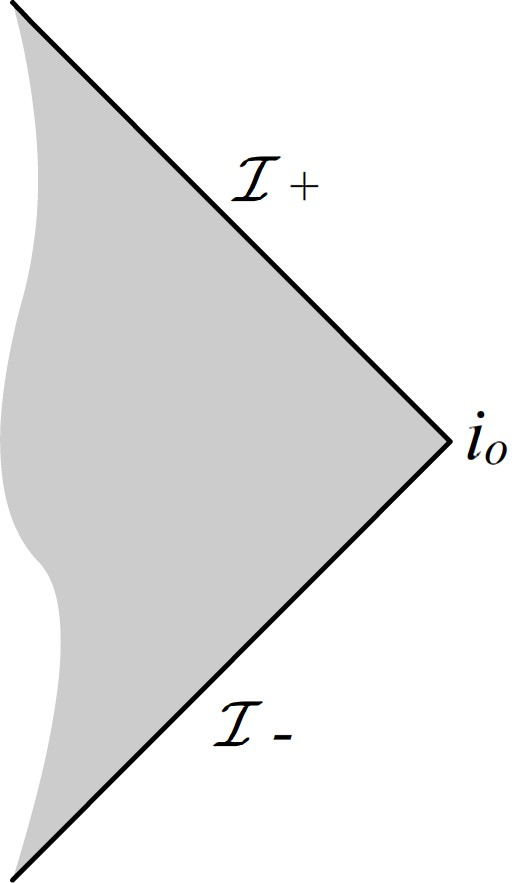
\includegraphics[scale=0.75] {fig18.jpg}
				\end{figure}
			\end{center}	
        \end{frame}
        
        \begin{frame}{Asymptotically Flat Manifold Diagram}
        	Asymptotically flat manifolds admit vectors that are asymptotically equivalent to the Killing vectors of Minkowski spacetime near $i_{0}$.\\
            \pause
            
            Therefore, these Killing vectors  allow the definition of total mass, momentum and angular momentum on spacelike hypersurfaces. 	
        \end{frame}
        
        \begin{frame}{Example 5: Kruskal Manifold}
           	Taking $\mathcal{M}$ as Kruskal's manifold \index{Kruskal} and $\tilde{\mathcal{M}}$
its conformal compactification, condition 3 above is NOT satisfied
because there are some null geodesics that end up at the singularity
and not in $\partial\tilde{\mathcal{M}}$.\\
\pause

Therefore, Kruskal is not asymptotically simple.\\
\pause

However, this manifold is weak asymptotically simple and asymptotically flat. Thus we conclude that it is also asymptotically flat as is shown in its Carter-Penrose diagram.
        \end{frame}
        
  	\begin{darkframes}
    
	\subsection{Causality Issues}
        \begin{frame}{Causal Curve}
			A \emph{causal curve }$\mathcal{C}\left(\lambda\right)$ is any non space-like smooth curve (i.e. it is time-like or null everywhere).
        \end{frame}
        
        \begin{frame}{Causal Past}
			The \emph{causal past} $\mathcal{J}^{-}\left(p\right)$ of point $p$
is the set of all the events that causally preceded point	$p$, i.e. is the set of all points $q$ for which there is at least	one future directed causal curve from $q$ to $p$.\\
			\bigskip
			\pause
			The causal past $\mathcal{J}^{-}\left(U\right)$ of a set of points $U\subset\mathcal{M}$ is the set of all points that causally preceded at least one point of $U$.
        \end{frame}
        
        \begin{frame}{Causal Future}
			The \emph{causal future} $\mathcal{J}^{+}\left(p\right)$ of a point $p$ is the set of all points $q$ for which there is at least one future directed causal curve from $p$ to $q$.\\ 
			\pause
			\bigskip
			The causal future $\mathcal{J}^{+}\left(U\right)$ of a set of points $U\subset\mathcal{M}$ is the set of all points that causally follow at least one point of $U$.
        \end{frame}
        
        \begin{frame}{Topological Closure}
			$\mathcal{\overline{J}}^{-}\left(U\right)$ and $\mathcal{\overline{J}}^{+}\left(U\right)$ are the topological closure of the causal past and causal future of $U$, respectively.
            \pause
            \bigskip
            
            $j^{-}\left(U\right)$ and $j^{+}\left(U\right)$ are the boundary of the topological closures, 

            \begin{eqnarray*}
            j^{-}\left(U\right) & = & \mathcal{\overline{J}}^{-}\left(U\right)-\mathcal{J}^{-}\left(U\right)\\
            j^{+}\left(U\right) & = & \mathcal{\overline{J}}^{+}\left(U\right)-\mathcal{J}^{+}\left(U\right).
            \end{eqnarray*}
        \end{frame}
        
        \begin{frame}{Future Event Horizon}
			The \emph{future event horizon }$\mathcal{H}^{+}$ is defined as the
boundary of the closure of the causal past of the null future infinite	$\mathcal{I}^{+}$.
			$$ \mathcal{H}^{+}=j^{-}\left(\mathcal{I}^{+}\right).$$        
		\end{frame}
        
        \begin{frame}{Past Event Horizon}
			Similarly, the \emph{past event horizon }$\mathcal{H}^{-}$ is defined
as the boundary of the closure of the causal future of the null past
infinite $\mathcal{I}^{-}$.
			$$\mathcal{H}^{-}=j^{+}\left(\mathcal{I}^{-}\right).$$   
		\end{frame}
  \end{darkframes}
        
        \begin{frame}{Example 6: Kruskal Manifold}
        	\begin{center}
				\begin{figure}
				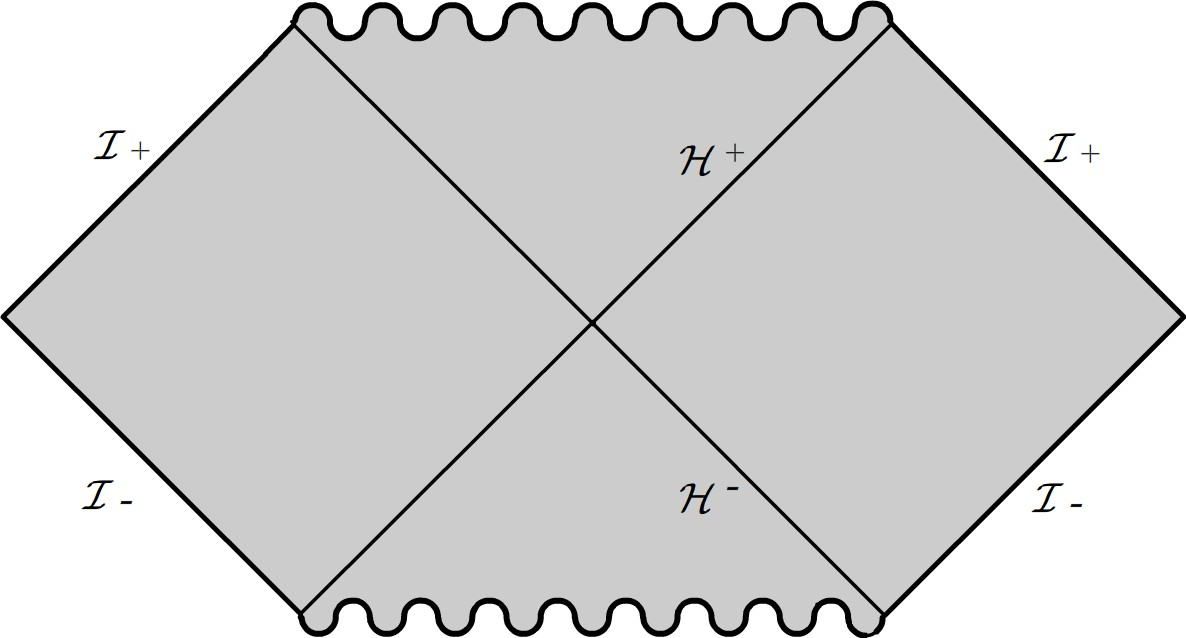
\includegraphics[scale=0.75] {fig19.jpg}
				\end{figure}
			\end{center}	
        \end{frame}
		 
  \begin{darkframes}
  		
        \begin{frame}{Black Hole}
			A \textit{Black Hole} in an asymptotically flat spacetime $\mathcal{M}$ is defined as the set of events that do not belong to the causal past of the future null infinity $\mathcal{J}^{-}\left( \mathcal{I}^{+} \right)$, namely
            $$ \mathcal{B} = \mathcal{M} - 
            \mathcal{J}^{-}\left( \mathcal{I}^{+} \right)$$
            \pause
            The \textit{event horizon} is the boundary of $\mathcal{B}$.
		\end{frame}
 	
    \end{darkframes}
        
        \begin{frame}{Example 6: Kruskal Manifold}
        	\begin{center}
				\begin{figure}
				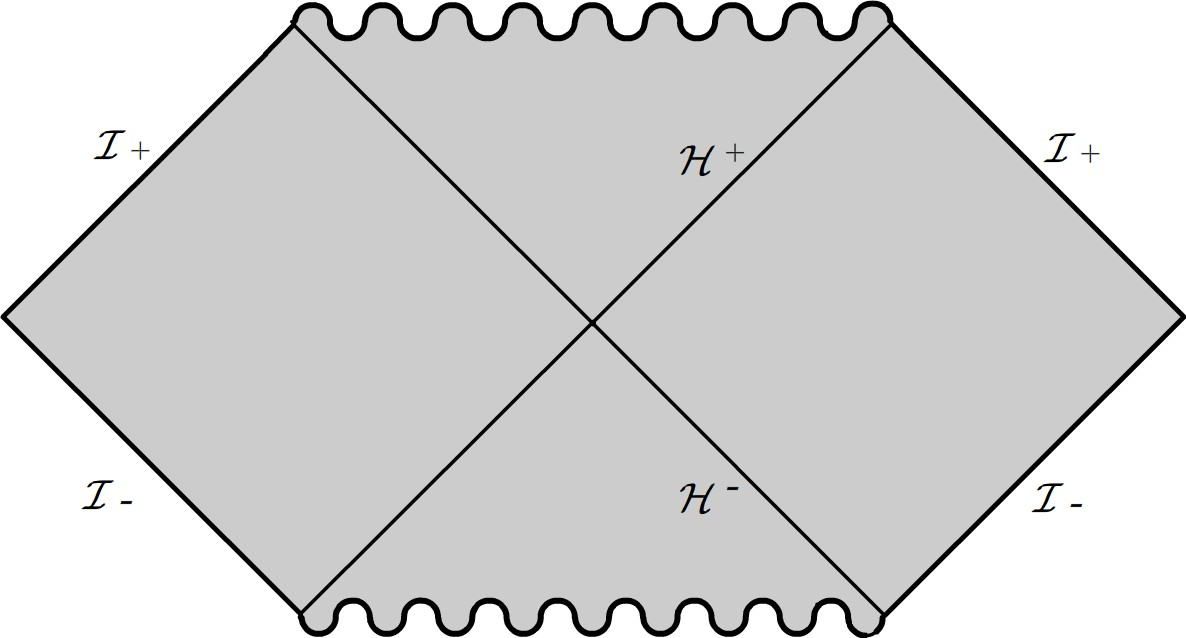
\includegraphics[scale=0.75] {fig19.jpg}
				\end{figure}
			\end{center}	
        \end{frame}
		 
  \begin{darkframes}    
  		\begin{frame}{Next Lecture}
        	\Large
			{05. Rotating Black Holes}
		\end{frame}
  
  \end{darkframes}
\end{document}
